\chapter{基于深度学习的文本情感分析}
\section{关于神经网络}
神经网络是一种模仿人类大脑运行模式设计的算法。神经网络由多个层(layer)组成,每层有多个神经元。运算在每个神经元中进行,通过数据在神经网络中流过模仿神经信号的传递。神经元中的运算一般会包括线性运算和一个非线性的激活函数,也有特殊的pooling层和dropout层。以一个全链接层(Full-connected layer的)为例,隐藏层中的每一个神经元接受上一层的所有输出作为它的输入$\textbf{x}$,在进行了线性运算$\textbf{w}* \textbf{x}+b$之后,经过一个非线性激活函数$f$,得到输出$f(\textbf{w} * \textbf{x} + b)$作为输入传到下一层。
\begin{figure}[ht]
\centering
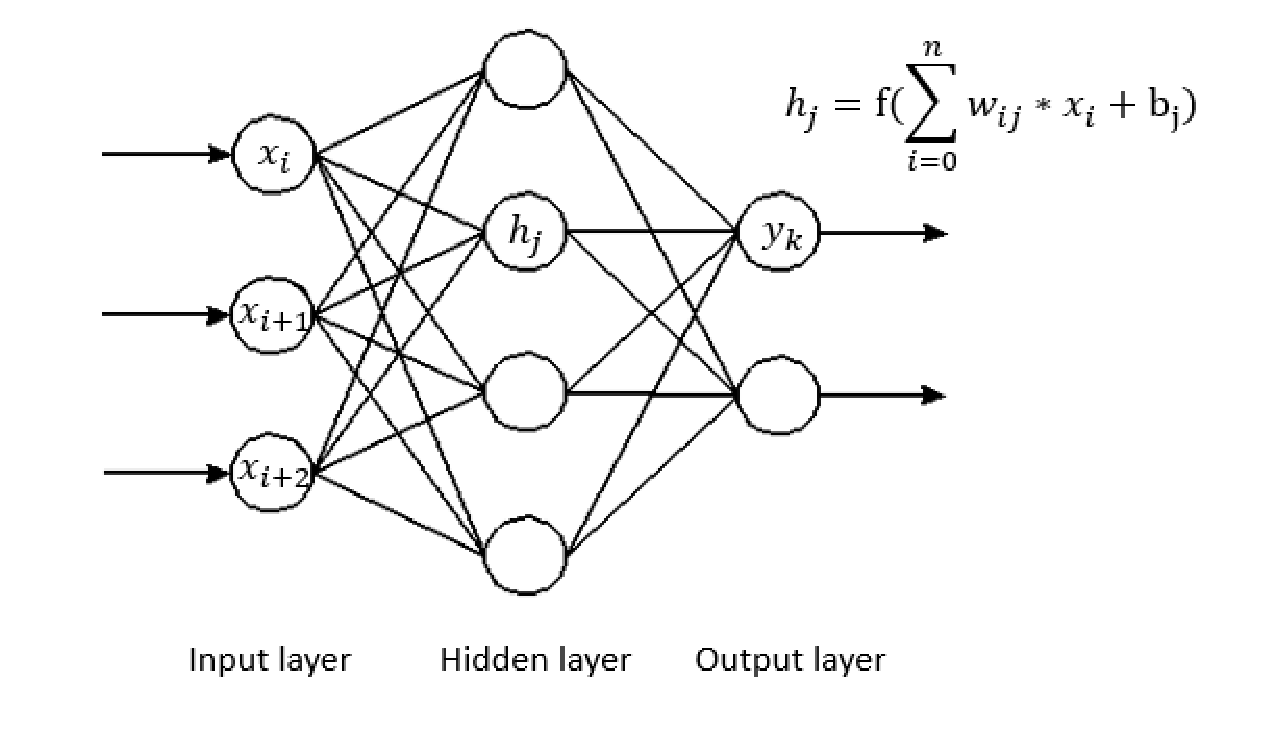
\includegraphics[width=15cm]{FullConnected}
\caption{一个单全链接隐藏层的神经网络} \label{fig:FullConnected}
\end{figure}

神经网络具有非常强的表达能力,具有一个隐藏层的神经网络,在有足够多的神经元数目时可以模仿任意的函数(函数的值域必须在一个有限的区间内)。故近年来神经网络被广泛应用于模式识别、分类等领域,得到了广泛的研究,涌现了如卷积神经网络、复发神经网络等网络结构。通过词嵌入的方法,可以将单词表示为一个固定维数的向量,从而让文本数据可以作为神经网络的合适输入,这样神经网络也可以用于像文本分类这样的问题中。


\section{词嵌入}
对于图像、声音相关的任务,一般都是处理稠密的、高维的输入数据,例如图像数据的像素级别的数据。但涉及到自然语言处理的问题时,传统的方法只能将每个单词表达为一个离散的原子的符号,如“猫”这个词表示为Id234,“狗”这个词表示为Id245。这样的表达只包含很少的信息,且忽视了不同单词间可能存在的关系,如 “猫”和“狗”会被认为是没有关系的两个符号。这样的表达方法还会导致数据非常稀疏,进一步导致需要很多的数据量才能成功训练出统计模型。

词嵌入(word embedding)可以很好地解决上述的问题。词嵌入指将单个词语映射到高维特征空间(一般100到300维)的一个向量。单词之间的相互关系在词向量中可以得到体现,两个单词的相似度一般可以通过计算其词向量的cosine相似度得出。进行词嵌入的算法有两种:基于计数的方法在一个大的语料里统计出一些单词和它的邻居互相同时出现的次数然后将统计结果映射到一个小的、稠密的向量中;预测模型则是建立一个直接从一个词的邻居中预测出这个词的模型,在这个模型的过程中训练出一个最优的词向量。

Word2vec是一种常用的高效率的词嵌入的算法,它是基于预测模型的算法,有Skip Gram和Continuous Bag of Word两种算法供选择,其区别在于预测模型的结构不同。本课题的词嵌入是使用Word2Vec训练出来的。

\section{卷积神经网络}
\subsection{卷积神经网络的结构}
卷积神经网络(Convolutional Neural Network,简称CNN)是一种特殊的神经网络结构,最初被应用在计算机视觉的领域。因为其模型结构非常适合图像数据的特征,卷积神经网络在计算机视觉领域取得了巨大成功,近年来,也被应用于自然语言处理领域的语义理解、语言模型、文本分类等问题上。

与全链接的神经网络层不同,卷积层的每个神经元并不以上一层的全部输出作为输入,而是只取局部的输出。卷积神经网络使用卷积核(convolutional kernels,又称为过滤器filters),每个卷积核只对应很小的感知域(receptive fields,大小可以为2 * 2, 3 * 3等),但这个感知域会贯穿输入数据的深度(输入的第三维,对应图像数据的channel)。对于图像数据而言,第一层卷积隐藏层的每一个神经元,只对应对应图像输入的一个小的像素块,其大小等于卷积核的尺寸,包含全部的RGB三通道。这样的一个神经元只包含其感知域的输入数据的权重参数,只处理输入数据中的一小块局部数据并产生它的输出。

卷积层的另一个特点是参数共享。对于同一个卷积核的全部神经元,其参数是相同的,故卷积神经网络可以理解为一个卷积核在输入数据上进行“滑动”,不断进行卷积运算并产生一个二维的输出。由于每个卷积层一般会有多个卷积核(同一大小的卷积核可以有多个,随机初始化它们的参数以训练出不同的卷积核),所以每个卷积层都会接受一个三维的输入,并给出一个三维的输出(多个卷积核的输出结果叠加形成第三维)。这样,一个卷积层的输出在经过线性整流层(Rectified Linear Units layer, ReLU layer)作非线性化处理后,可以很方便地作为输入进入下一个卷积层。

卷积神经网络层相较于全链接层的一个优势在于不会有“纬度诅咒”的问题。例如,对于一个100*100*3的输入数据(图像数据或者经过词嵌入的文本数据都有这样的结构),在第一个隐藏全链接层中的每一个神经元都需要有 100 * 100 * 3 = 30000个权重参数,如果该层有100个神经元,则会产生100 * 30000 = 3000000个权重参数。而对于一个有128个2 * 2的卷积核的卷积层,只需要2 * 2 * 3 * 128 = 1536个权重参数 。
卷积神经网络的另一个优势在于可以提取输入数据的局部特征,每个卷积核只处理输入数据的一小块,多层卷积层后,图像数据的信息得到更好的归纳。

\subsection{卷积神经网络应用于文本问题}
卷积神经网络在计算机视觉领域的成功与图像数据的结构特点密切相关。与图像数据由像素点组成不同,文本数据由单词组成,因此,卷积神经网络不能直接应用于文本数据上。必须将文本数据映射成一个维度不高、稠密的矩阵数据形式。

通过对文本数据进行词嵌入,我们可以用一个句子中所有单词的词向量拼接出一个二维的矩阵。使用多个不同的词嵌入(要求词向量的维度相同),可以得到多个这样的二维数据,从而堆叠出一个三维的数据(第三维对应图像数据中的channel)。这样,文本数据转化成为卷积神经网络可以接受的输入。

应用于文本数据输入的卷积神经网络与图像数据的卷积神经网络存在着一些差别,主要在于卷积核的大小。应用于图像数据的卷积神经网络卷积核大小可以为2 * 2,3 * 3,2 * 3等,长和宽没有严格的限制。但对于接受文本数据输入的卷积层,其卷积核的宽度一般等于词向量的宽度,即卷积核会占满词向量这一维,只在句子长度这一维上滑动。这是因为每一行都是原输入数据中的一个单词,如果在单词内部使用更小的卷积核进行卷积运算的话,相当于“破开”了一个单词。在不了解词向量每一位的意义的情况下,“破开”词向量并不合理。此外,卷积核的长度(对应每次进行卷积运算时覆盖的单词数)也不会太长,一般很少会超过五。因为文本中每个单词相较于图像中的像素,粒度要大一些,如果卷积核的感知域覆盖了太多单词,就不存在“提取局部特征”的优势了。

应用于文本领域的卷积神经网络与传统的n-gram方法有相似之处,它们都会提取连续出现的单词作为句子或者文档的局部特征。相较于传统的n-gram方法,卷积神经网络有如下几个优势:首先卷积神经网络不用像n-gram那样建立非常大的词典(在比较大的语料上,3-gram已经需要建立庞大的词典才能正常工作);此外,卷积神经网络可以利用GPU的硬件优势,进一步得到加速,因为卷积运算作为一个计算机图形学中非常基础的运算,通常在GPU的硬件层面上就会给予特别支持。

\begin{figure}[ht]
\centering
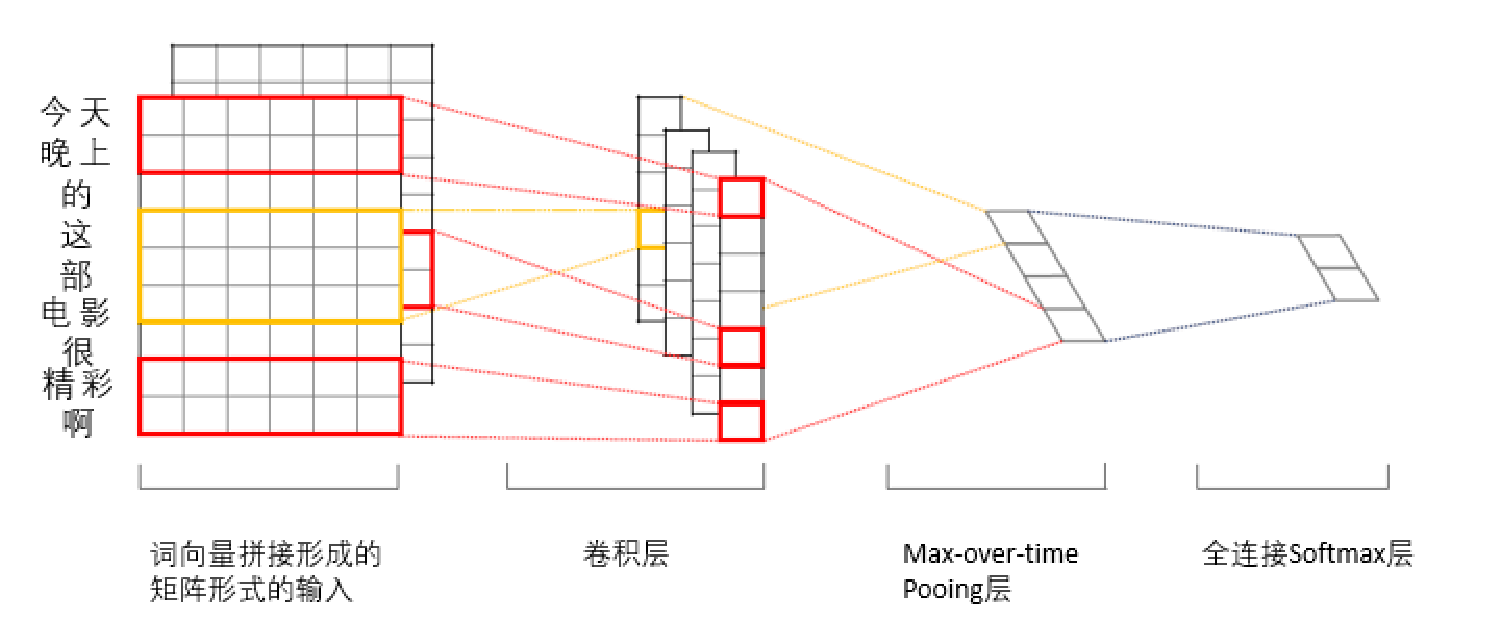
\includegraphics[width=15cm]{CNN}
\caption{卷积神经网络应用于文本分类,图像部分引用自\cite{kim.2014.convolutional}} \label{fig:CNN}
\end{figure}

\subsection{具体算法}
用$w_i\in \mathbf{R}^k$来表示句子中的第i个单词对应的长度为$k$的词向量,一个长度为n的句子可以表示为:
\begin{equation} \label{eq3.1}
x_{1:n} = [x_1; x_2;...; x_n]
\end{equation}
使用$x_{i:i+j}$来表示词向量$x_i, x_{i+1}, …, x_{i+j}$连接的结果。一个卷积核$w\in \mathbf{R}^{h*k}$,将作用在一个包含h个单词的“窗口”上来产生一个特征。例如,一个特征$c_i$可以从单词$w_{i:i+h-1}$中通过下式产生:
\begin{equation} \label{eq3.2}
c_i = f(\textbf{w}*\textbf{x}_{i:i+h-1} + b)
\end{equation}	
这里的$b$为偏差值(bias),$f$是一个非线性函数(如ReLU)。随着窗口在整个句子上滑动,这个卷积核可以作用在每一个可能的窗口上,产生了如下的特征序列:
\begin{equation} \label{eq3.3}
\textbf{c} = [c_1, c_2, ..., c_{n-h+1}]
\end{equation}	
$\textbf{c}\in\mathbf{R}^{n-h+1}$。在卷积层得到的特征序列上加以一个max-over-time pooling,只保留特征序列中的最大值\^{c}=$max\{\textbf{c}\}$,这是为了只保留每个特征序列中最重要的特征。在经过max-pooling层后,每个卷积核只保留了一个特征。多数个卷积核(可以有不同的窗口大小)会产生一系列的特征,这些特征连接起来,作为最后的全连接Softmax层的输入。
此外,在输入层和max-pooling层之后,我们的模型中加入两个dropout层。Dropout层会随机地筛选出一部分输入,将其值设为0,再进行输出。Dropout层的目的是通过随机去掉一些神经网络中的信号传递以减少过拟合。

\section{复发神经网络}
复发神经网络(Recurrent Neural Network,简称RNN)是另一个常见的神经网络结构,复发神经网络中的信号不仅会向前传播,而且会传回给自身,因此被称为recurrent。具体到文本问题上,复发神经网络单元每次在处理完一个单词后,除去产生一个输出外,还会记住一部分信息。在处理下一个单词时,会根据当前输入以及之前记住的信息来产生下一个输出,并更新记住的信息。

Long Short Term Memory,简称LSTM,是一种特殊的复发神经网络。它使用一个“遗忘门”来选择性的忘记一部分记住的信息,同时使用一个“输入门”来记住一部分非线性话处理后的上一轮留下的输入。LSTM的优势在于他可以处理长距离的依赖关系。

复发神经网络由于能够在文本数据流过网络时“记住”一些之前的信息,因此,可以很好利用到输入数据的全局特征和顺序特征。在文本分类这个问题上,他可以利用词语的位置特征,挖掘整个句子的信息。复发神经网络在文本相关的问题上一直有很好的表现。

由于本课题只使用LSTM作为一个用于比较的实验,重点仍然是卷积神经网络在情感分析问题上的应用,故只简单地介绍LSTM的原理。关于RNN和LSTM的具体内容,可以参考\cite{socher.2013.recursive}和\cite{sundermeyer2012lstm}。

\section{小结}
本章对深度学习的方法如何应用于情感分析问题进行了说明。首先简介了神经网络的基本原理,然后词嵌入技术进行了说明;之后对就卷积神经网络相关内容进行了详细介绍包括其原理、如何应用于文本问题以及具体的算法;最后简介了作为baseline实验的LSTM的基本原理。
